\section{Introduction}
It is the main goal of this experiment to understand the mode of operation of an
ideal and a real operational amplifier.

\section{Theory}
\FloatBarrier
\begin{figure}
  \centering
  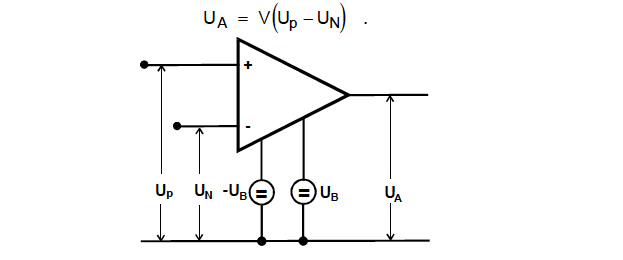
\includegraphics[scale=0.5]{opamp.PNG}
  \caption{Circuit of an operational amplifier. \cite{Q1}}
  \label{abb1}
\end{figure}
\FloatBarrier
The picture above shows the circuit of an ideal operational amplifier. It is
fed with two constant voltages $U_{\text{B}}$ and -$U_{\text{B}}$.
Further the operational amplifier has two inputs, an inverting ($-$) and a
non-inverting ($+$) one. The output voltage $U_{\text{A}}$ is calculated by:
\begin{align}
    U_{\text{A}} = V(U_{\text{p}}-U_{\text{N}}) \ .
    \label{eq:outputvoltage}
\end{align}
Where $U_{\text{p}}$ represents the voltage going into the non-inverting ,
$U_{\text{N}}$ the one going into the inverting input and $V$, the proportionality
factor is the open loop gain of the operational amplifier.
The output voltage is only amplified while the output voltage lies within the
modulation range:
\begin{align*}
    -U_{\text{B}} < U_{\text{A}} < U_{\text{B}} \ .
\end{align*}
Outside of this interval the output voltage $U_{\text{A}}$ equals the operational
voltage $\pm U_{\text{B}}$. The saturation curve can be seen in the figure \ref{abb2}.
\FloatBarrier
\begin{figure}
  \centering
  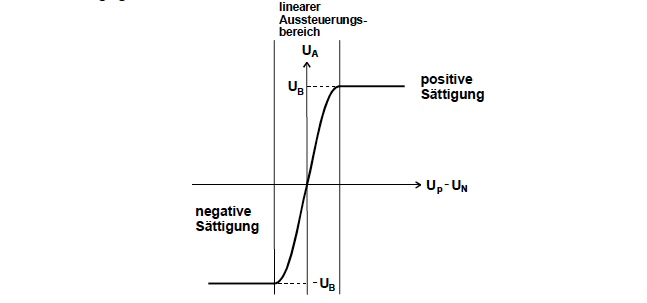
\includegraphics[scale=0.5]{saturation.PNG}
  \caption{Characteristic curve of an operational amplifier. \cite{Q1}}
  \label{abb2}
\end{figure}
\FloatBarrier

\noindent In order to describe an operational amplifier correctly it is important to define
a few more parameters such as the two input resistances $r_{\text{e}_{{}_\text{p}}}$
and $r_{\text{e}_{{}_\text{N}}}$ and the output resistance $r_{\text{a}}$.
Usually the open loop gain $V$ is very high and dependent on the frequency of the
input voltage, in the case of an ideal operational amplifier it is considered to
be infinite. The same applies to the two input restistances. They are usually very
high and are considered to be infinite when talking about the ideal operational
amplifier. The output restistance is to be kept as small as possible which is why
it is considered to be zero for the ideal case.
\begin{align*}
    V_{\text{id}}=\infty,~ r_{\text{e}_{\text{id}}}=\infty,~ r_{\text{a}_{\text{id}}}=0
\end{align*}
Regarding a real operational amplifier some assymetrics in the amplifying inputs
have to be taken into consideration which is why the output voltage is unequal to
zero even when the two input voltages $U_{\text{Gl}}$ are the same. This is
called the common mode gain. In this case the common mode amplification is described
as:
\begin{align*}
    V_{\text{Gl}}:=\frac{\Delta U_{\text{A}}}{\Delta U_{\text{Gl}}}.
\end{align*}
Due to the fact that the real input resistances cannot be infinite there will occur
input currents, $I_{\text{p}}$ and $I_{\text{N}}$, that are unequal to zero.
The overall input current is described as follows:
\begin{align*}
    I_{\text{B}} = \frac{1}{2} \left( I_{\text{p}} + I_{\text{N}} \right).
\end{align*}
Further the difference betweeen the two input currents is called offset current
and can be described as:
\begin{align*}
    I_0:=I_{\text{p}} - I_{\text{N}} ,~ \text{ with } U_{\text{N}} = U_{\text{p}} = 0 .
\end{align*}
With the two input currents $I_{\text{p}}$ and $I_{\text{N}}$ it is now possible
to calculate the differential input impedance:
\begin{align*}
    r_\text{D}:=
	\begin{cases}
		\frac{\Delta U_{\text{p}}}{\Delta I_{\text{p}}} ~ \text{, while }~ U_{\text{N}} = 0   \\
		\\
		\frac{\Delta U_{\text{N}}}{\Delta I_{\text{N}}} ~ \text{, while }~ U_\text{p}=0
\end{cases}
\end{align*}
As well as the common mode input impedance:
\begin{align*}
    r_{\text{Gl}} = \frac{\Delta U_{\text{Gl}}}{\Delta I_{\text{Gl}}}
\end{align*}
In this equation $U_{\text{Gl}}$ is equal to $U_{\text{p}}$ and $U_{\text{N}}$ and
$I_{\text{Gl}}$ is calculated by the addition of $I_{\text{p}}$ and $I_{\text{N}}$.

\noindent For a real operational amplifier the output voltage is often unequal to zero while
$U_{\text{p}} = U_{\text{N}} = 0$, eventhough this could be concluded from equation
\ref{eq:outputvoltage}.
Therefore an offset voltage $U_0$ is defined as the voltage difference that has to
be set between the two input voltages so the output voltage dissapears:
\begin{align*}
    U_0 := U_{\text{p}} - U_{\text{N}} ,~ \text{ for } U_{\text{A}}=0
\end{align*}
All the above currents and voltage dissapear in the case of the ideal operational
amplifier and the impedances $r_{\text{D}}$ and $r_{\text{Gl}}$ are considered to
be infinite.

\subsection{Linear amplifier}
Due to the already mentioned very high open loop gain $V$ it is impossible to use
an operational amplifier as a linear amplifier without making any modifications to
the circuit. The modified circuit is displayed in figure \ref{abb3}. The difference
to figure \ref{abb1} is the degenerative feedback which puts a part of the output
voltage back to the inverting input. This leads to a decrease of the input voltage if
the output voltage gets bigger.
\FloatBarrier
\begin{figure}
  \centering
  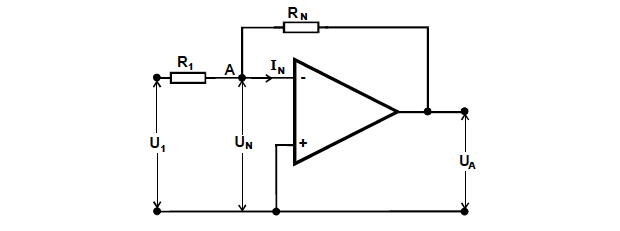
\includegraphics[scale=0.5]{degenerative.PNG}
  \caption{Circuit of the degenerative inverting amplifier. \cite{Q1}}
  \label{abb3}
\end{figure}
\FloatBarrier
The high value for the open loop gain is also the reason for the fact that the
voltage that goes into the inverting input is approxiamtely zero:
\begin{align*}
    U_{\text{N}} = - \frac{U_{\text{A}}}{V}
\end{align*}
as well as the input current $I_{\text{N}}$ because the input impedance is extremely
high.
In the circuit shown in figure \ref{abb3} the amplification factor $V$ for an ideal
oerational amplifier can be calculated according to the Kirchhoff Current Law
applied to point A in the figure:
\begin{align}
    V'=-\frac{\text{R}_{\text{N}}}{\text{R}_1}.
    \label{eq:ampfactor}
\end{align}
In order to calculate the amplification factor $V'$ for an ideal operational amplifier
the following equation is used:
\begin{align}
    \frac{1}{V'} \approx \frac{1}{V} + \frac{\text{R}_1}{\text{R}_{\text{N}}}
    \label{eq:ampfactor_real}
\end{align}
Taking a look at the equation \ref{eq:ampfactor_real} it can be seen that $V'$ has
the same value in \ref{eq:ampfactor} as in \ref{eq:ampfactor_real} in the case of
$R_{\text{N}}/R_1 \ll V$.
The fact that the amplification $V'$ is modified by the outer resistance and the
relation between $R_{\text{N}}$ and $\text{R}_1$ makes the amplifier independent from
influences coming from the outside for example temperature which could influence $V$.
Therefore by including the negative feedback into the circuit the linear amplifier becomes
much more stable.
At the same time the output resistance $r_{\text{a}}$ is decreased by the factor
of $g$:
\begin{align*}
    g:= \frac{V}{V'}.
\end{align*}
The influence of possible variations in the open loop gain on the amplification
factor $V'$ are also reduced by the factor $g$:
\begin{align*}
    \frac{\Delta V'}{V'}=\frac{1}{g}\frac{\Delta V}{V}.
\end{align*}
Finally the bandwidth of the operational amplifier is broadened by the factor of
$g$ which means that higher frequencies are transmitted wihtout distortion as shown
in figure \ref{abb4}. The highest freuquency that is transmitted without distortion
is called cut off frequency. The amplification factor $V'$ has decreased to a value of
1 and the amplifier does not show a linear behaviour anymore.
\FloatBarrier
\begin{figure}
  \centering
  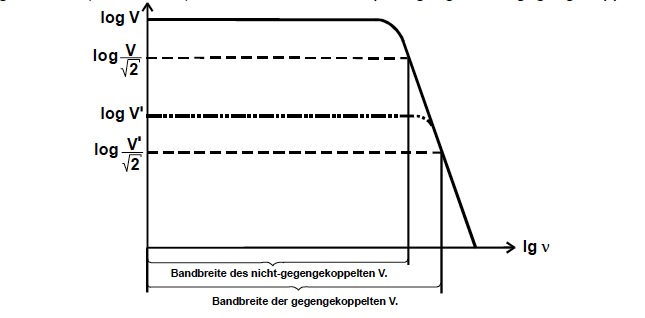
\includegraphics[scale=0.5]{bandwidth.PNG}
  \caption{Frequency response of an operational amplifier. \cite{Q1}}
  \label{abb4}
\end{figure}
\FloatBarrier

\subsection{Reverse Integrator}
If the resistance in the circuit shown in \ref{abb3} is replaced by a capacitor \textbf{C}
as shown in \ref{abb5} the operational amplifier can be used as a reverse integrator
of the input signal so the output signal can be calculated by:
\begin{align*}
    U_{\text{A}} = -\frac{1}{\text{RC}} \int U_1(t) dt
\end{align*}
The '-' in the above formula is the reason for the integrator being called a reverse
integrator and $U_{\text{N}} \approx 0$.
It can be seen that the amplitude of the output voltage depends on the inverse frequency
of the input voltage.
\FloatBarrier
\begin{figure}
  \centering
  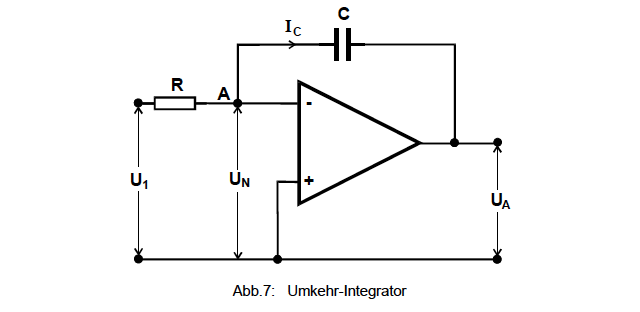
\includegraphics[scale=0.5]{integrator.PNG}
  \caption{Circuit of a reverse integrator. \cite{Q1}}
  \label{abb5}
\end{figure}
\FloatBarrier

\section{Experiment set-up}
The circuits that are previously described can be easily built up on an electrical
pin board. At the sight of the experiment is a short explanation of the various inputs
of the operational amplifier, various resistances, capacitors as well as a voltage generator which is able to
generate sine-, cosine-, triangle- or rightangle- voltages that can be fed into the
input of the operational amplifier.

\section{Lead-through}

In the first part of the experiment the circuit from figure \ref{abb3} is used to
figure out the characteristic roll off and although the cut-off frequency of the
operational amplifier that is used. Therefore a constant fed of the operational
amplifier of $\SI{12}{\volt}$has to be guaranteed for each part of the experiment.
As soon as the circuit from figure \ref{abb3} is set up the frequency of the input
sine-voltage is increased from $\SI{10}{\hertz}$ up to $\SI{1}{\mega \hertz}$ for
two different set ups of resistances.
The second part of the experiment includes the circuit of the reverse integrator as
shown in figure \ref{abb5}. In the first subsection the picture shown in the oscilloscope
is analyzed in regard to the fact that an integration if the input voltage is expected.
Afterwards the frequency of the input voltage is increased from $\SI{570}{\hertz}$
to $\SI{16}{\kilo \hertz}$ in order to show that with an increase of the input frequency
the output voltage tends to a certain value.
